\documentclass{beamer}

\usetheme{Dresden}
\usecolortheme{beaver}

\usepackage{listings}
\usepackage[utf8]{inputenc}
\usepackage[french]{babel}
\usepackage{xcolor,colortbl,verbatim}
\beamertemplatenavigationsymbolsempty

\let\emph\alert

\lstdefinelanguage{ocaml}
{
basicstyle=\ttfamily,
morekeywords=[1]{val,type},%
keywordstyle=[1]{\color{red}},%
%morekeywords=[2]{true,false},%
%keywordstyle=[2]{\color{blue}},%
otherkeywords={},%
commentstyle=\itshape,%
columns=[l]fullflexible,%
sensitive=true,%
morecomment=[s]{(*}{*)},%
escapeinside={*?}{?*},%
keepspaces=true,
literate=%
{<}{$<$}{1}%
{>}{$>$}{1}%
{<=}{$\le$}{1}%
{>=}{$\ge$}{1}%
{<>}{$\ne$}{1}%
{->}{$\rightarrow$}{2}%
{<-}{$\leftarrow$}{2}%
{<->}{$\leftrightarrow$}{2}%
%
%
}

\lstnewenvironment{ocaml}{\lstset{language=ocaml}}{}

\lstdefinelanguage{combine}
{
basicstyle=\ttfamily,
morekeywords=[1]{pattern, tiles, problem, count, set},%
keywordstyle=[1]{\color{red}},%
keepspaces=true,
columns=[l]fullflexible,%
sensitive=true,%
}
\lstnewenvironment{combine}{\lstset{language=combine}}{}


\begin{document}

\author{Rémy El Sibaïe Besognet \\
Jean-Christophe Filliâtre}
\title{\texttt{combine} : \\ une bibliothèque OCaml pour la combinatoire}
\date{JFLA 2013}

\begin{frame}
  \titlepage
\end{frame}

\begin{frame}\frametitle{Pavage}
  \begin{center}
  \only<1>{\includegraphics{imports/caml_problem.mps}}%
  \only<2,3>{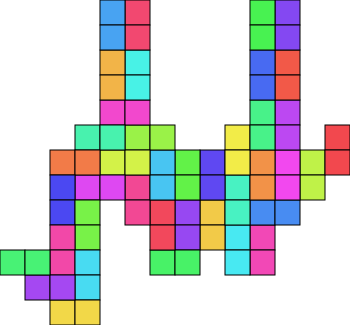
\includegraphics{imports/caml_solution.mps}}%
  \only<4,5>{\includegraphics{imports/caml2_problem.mps}}%
  \\[2em]
  \only<3>{46\,976 solutions}%
  \only<5>{32\,420\,116\,341\,024\,288 solutions}
  \end{center}
\end{frame}

%%% 1 EMC
\begin{frame}{Couverture exacte de matrice (EMC)}

  soit une matrice contenant des 0 et des 1

  \bigskip

  \begin{displaymath}
   \left(\begin{array}{ c c c c c }
   1 & 0 & 1 & 1 \\
   0 & 1 & 1 & 0 \\
   1 & 1 & 0 & 1 \\
   1 & 0 & 0 & 1 \\
   0 & 1 & 0 & 0
  \end{array}\right)
  \end{displaymath}

  \bigskip

  on cherche un sous-ensemble de lignes \par
  avec un 1 et un seul par colonne

  % TODO : donner les solutions (et les non solutions) à l'oral
  % problème difficile
\end{frame}

% le faire à l'oral
% \begin{frame}{EMC : exemple}

% \begin{displaymath}
%    \left(\begin{array}{ c c c c c }
%    1 & 0 & 1 & 1 \\
%    0 & 1 & 1 & 0 \\
%    1 & 1 & 0 & 1 \\
%    1 & 0 & 0 & 1 \\
%    0 & 1 & 0 & 0
%   \end{array}\right)
%   \end{displaymath}

% \begin{center}
% $ \{3, 4\} $ n'est pas une solution\\
% $ \{0, 4\}, \{1, 3\} $ sont des solutions
% \end{center}
% \end{frame}

\begin{frame}\frametitle{Applications}
  de nombreux problèmes peuvent se ramener à EMC

  \bigskip
  exemples :
  \begin{itemize}
  \item pavage
  \item N-reines
  \item Sudoku
  \item coloriage de graphe
  \end{itemize}
\end{frame}


\begin{frame}{Exemple : pavage avec des dominos $2\times 1$}

  colonnes = cases à paver

  lignes = différentes façons de poser un domino

  \begin{center}
    \includegraphics{imports/caml_problem.mps}
  \end{center}

  \begin{center}
    1 ~ 1 ~ 0 ~ 0 ~ 0 ~ 0 ~ 0 ~ 0 ~ 0 ~ 0 ~ 0 ~ 0 ~ 0 ~ 0 ~ 0 ~ 0 ... \\
    0 ~ 0 ~ 1 ~ 1 ~ 0 ~ 0 ~ 0 ~ 0 ~ 0 ~ 0 ~ 0 ~ 0 ~ 0 ~ 0 ~ 0 ~ 0 ... \\
    0 ~ 0 ~ 0 ~ 1 ~ 1 ~ 0 ~ 0 ~ 0 ~ 0 ~ 0 ~ 0 ~ 0 ~ 0 ~ 0 ~ 0 ~ 0 ... \\
    $\vdots$
  \end{center}
\end{frame}



% \begin{frame}{Application : Sudoku}

% \begin{figure}[h]
% \scalebox{0.7}{
% \centering

% $\begin{array}{|c|c|c||c|c|c||c|c|c|}
% \hline
% 5 & 3 &   &   & 7 &   &  &   &    \\
% \hline
% 6 &   &   & 1 & 9 & 5 &  &   &    \\
% \hline
%   & 9 & 8 &   &   &   &  & 6 &    \\
% \hline
% \hline
% 8 &   &   &   & 6 &   &   &   & 3 \\
% \hline
% 4 &   &   & 8 &   & 3 &   &   & 1 \\
% \hline
% 7 &   &   &   & 2 &   &   &   & 6 \\
% \hline
% \hline
%   & 6 &   &   &   &   & 2 & 8 &   \\
% \hline
%   &   &   & 4 & 1 & 9 &   &   & 9 \\
% \hline
%   &   &   &   & 8 &   &   & 7 & 5 \\
% \hline
% \end{array}$
% }
% \end{figure}

% 324 colonnes :
% \begin{enumerate}
% \item 81 cases
% \item $ 9~\textrm{lignes} \times 9~\textrm{valeurs}$
% \item $ 9~\textrm{colonnes} \times 9~\textrm{valeurs}$
% \item $ 9~\textrm{cellules} \times 9~\textrm{valeurs}$
% \end{enumerate}

% \[
% 	0 0 \dots 1 \dots 0 | 0 0 \dots 1 \dots 0 |
% 	0 0 \dots 1 \dots 0 | 0 0 \dots 1 \dots 0
% \]


% \end{frame}




% \begin{frame}{Application : N-Reines}
% \begin{figure}[h]
% \begin{center}
% 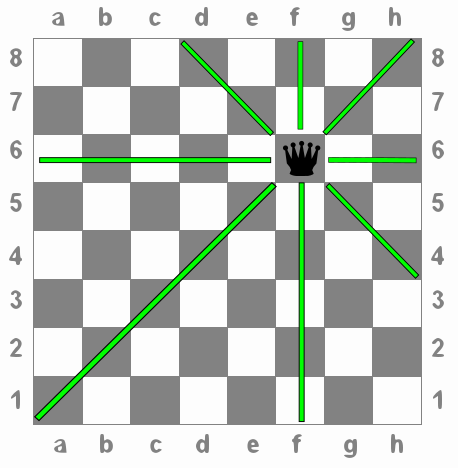
\includegraphics[height=0.4\textheight]{imports/8queens.pdf}
% \end{center}
% \end{figure}

% 46 colonnes :
% \begin{itemize}
% \item 8 lignes
% \item 8 colonnes
% \item 15 diagonales gauche-droite
% \item 15 diagonales droite-gauche
% \end{itemize}
% \[
% 	0 0 \dots 1 \dots 0 | 0 0 \dots 1 \dots 0 |
% 	\textcolor{red}{0 0 \dots 1 \dots 0} | \textcolor{red}{0 0 \dots 1 \dots 0}
% \]

% \end{frame}

\begin{frame}[fragile]\frametitle{Interface}
  \begin{ocaml}
  type t

  val create: ?primary:int -> bool array array -> t

  type solution = int list

  val iter_solution: (solution -> unit) -> t -> unit
  val get_first_solution: t -> solution
  val count_solutions: t -> int
  \end{ocaml}
\end{frame}


\begin{frame}{Deux techniques pour résoudre EMC}

  \begin{itemize}
  \item les liens dansants (DLX)
  \item les \textit{Zero-Suppressed BDDs} (ZDD)
  \end{itemize}

\end{frame}



%%% 2 DLX
\begin{frame}{Les liens dansants (DLX)}

  Donald Knuth, \emph{Dancing links} \par
  {\small(Millenial Perspectives in Computer Science, 2000)}

  \bigskip\bigskip

  une utilisation astucieuse des listes doublements chaînées :

  \medskip
  \begin{center}
    % TODO faire plutôt 2 figures
    \includegraphics[scale=0.35]{imports/delete.png}
  \end{center}
\end{frame}

% \begin{frame}{Principe de base de DLX}
% Suppression puis ré-ajout
% \begin{figure}[h]
% \begin{center}
% \includegraphics[scale=0.3]{imports/delete.png}
% \end{center}
% \end{figure}
% \end{frame}

\begin{frame}{Les liens dansants (DLX)}
 \begin{columns}
    \column{0.5\textwidth}
  \begin{displaymath}
   \left(\begin{array}{ c c c c c }
   1 & 0 & 1 & 1 \\
   0 & 1 & 1 & 0 \\
   1 & 1 & 0 & 1 \\
   1 & 0 & 0 & 1 \\
   0 & 1 & 0 & 0
  \end{array}\right)
  \end{displaymath}

    \column{0.5\textwidth}
    \includegraphics[width=0.8\textwidth]{imports/dlx.mps}
 \end{columns}
\end{frame}

\begin{frame}{Les liens dansants (DLX)}
  \begin{columns}
  \column{0.5\textwidth}
  \begin{displaymath}
   \begin{array}{ccccc} \\
   &
   \only<2-10>{\downarrow} &
   \only<7,8,10>{\downarrow} &
   \only<5-7,10>{\downarrow} &
   \only<5-10>{\downarrow}
   \\
   \only<4-7>{\rightarrow} &
   \only<4-7>{\cellcolor{red}} 1 &
   0 &
   \only<3,8-10>{\cellcolor{gray}}\only<4-7>{\cellcolor{red}} 1 &
   \only<3,8-10>{\cellcolor{gray}}\only<4-7>{\cellcolor{red}} 1
   \\
   & 0 &
   \only<5-8>{\cellcolor{gray}}\only<10>{\cellcolor{red}} 1 &
   \only<5-8>{\cellcolor{gray}}\only<10>{\cellcolor{red}} 1 & 0
   \\
   \only<8>{\rightarrow} &
   \only<8>{\cellcolor{red}} 1 &
   \only<3-7,9-10>{\cellcolor{gray}}\only<8>{\cellcolor{red}} 1 &
   0 & \only<3-7,9-10>{\cellcolor{gray}}\only<8>{\cellcolor{red}} 1
   \\
   \only<9-10>{\rightarrow} &
   \only<9-10>{\cellcolor{red}} 1 &
   0 &
   0 &
   \only<3-8>{\cellcolor{gray}}\only<9-10>{\cellcolor{red}} 1
   \\
   & 0 &
   \only<7>{\cellcolor{red}} 1 & 0 & 0
  \end{array}
  \end{displaymath}

  \column{0.5\textwidth}
  \only<2>{on choisit une colonne}

  \only<3>{on la \emph{couvre} \par
           i.e. on efface les 1 sur les mêmes lignes que ses 1}

  \only<4>{on parcourt successivement ses 1}

  \only<5>{on couvre les colonnes de la ligne sélectionnée}

  \only<6>{on recommence tant qu'il reste des colonnes à couvrir}

  \only<7>{on obtient ici la solution \{0,4\}}

  \only<8>{on \textit{backtrack} et on passe au 1 suivant de la
           première colonne

          \bigskip
          impossible de couvrir la troisième colonne $\Rightarrow$ pas
          de solution}

  \only<9>{on \textit{backtrack} encore et on passe au dernier 1 de la
           première colonne
          }

  \only<10>{une seule façon de couvrir la troisième colonne

    \bigskip
    donne la solution \{1,3\}}
  \end{columns}
\end{frame}


% \begin{frame}{Déroulement}
% 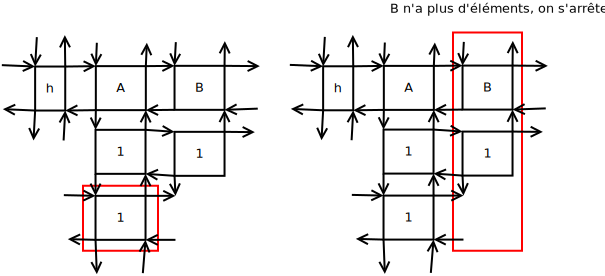
\includegraphics[scale=0.30]{imports/second_iter.pdf}
% \end{frame}

\begin{frame}{}
  \begin{center}
			Et maintenant... ZDD
  \end{center}
\end{frame}




%%% 3 ZDD
\begin{frame}{Zero-Suppressed Binary Decision Diagram (ZDD)}

  Shin ichi Minato (DAC, 1993)


  \begin{columns}
    \column{0.5\textwidth}
    ensemble d'ensembles d'entiers

    \bigskip\bigskip
    \bigskip\bigskip
    \{\{0, 1, 2\}, \{0\}, \{1\}, \{2\}\}

    \column{0.5\textwidth}
    \hspace*{-1em}\includegraphics[scale=0.5]{imports/zdd_ex.pdf}
  \end{columns}
\end{frame}


\begin{frame}{Comme pour les BDD}
  \begin{columns}
    \column{0.6\textwidth}
    \begin{itemize}
    \item partage maximal des sous-arbres
    \item ordre croissant des éléments
    \item pas de \textsf{Bot} à droite

    \bigskip
    \item opérations avec \emph{mémoïzation}
    \end{itemize}

    \column{0.4\textwidth}
    \includegraphics[scale=0.6]{imports/zdd_construct.pdf}
  \end{columns}
% \begin{center}
% \includegraphics[scale=0.3]{imports/zdd_ex.pdf}
% \end{center}
% \begin{itemize}
% \item Pas de $\bot$ à droite
% \item Valeur des n\oe uds croissante en descendant
% \end{itemize}
\end{frame}

\begin{frame}{EMC vers ZDD}
  \begin{columns}
    \column{0.5\textwidth}

    d'abord la couverture d'\emph{une} colonne

    \bigskip

  \begin{displaymath}
    \begin{array}{c}
      0. \\ 1. \\ 2. \\ 3. \\ 4.
    \end{array}
   \left(\begin{array}{ c c c c c }
   1 & 0 & 1 &\cellcolor{red} 1 \\
   0 & 1 & 1 &\cellcolor{red} 0 \\
   1 & 1 & 0 &\cellcolor{red} 1 \\
   1 & 0 & 0 &\cellcolor{red} 1 \\
   0 & 1 & 0 &\cellcolor{red} 0
  \end{array}\right)
  \end{displaymath}

  \bigskip
  \{\{0\},\{0,1\},\{0,4\},\{0,1,4\}, \par
  ~ \{2\},\{2,1\}, \dots \}

    \column{0.5\textwidth}
    \includegraphics[height=0.9\textheight]{imports/column.pdf}
  \end{columns}
\end{frame}

\begin{frame}{EMC vers ZDD}
  \begin{columns}
    \column{0.3\textwidth}

    on fait ensuite

    l'\emph{intersection}

    de tous ces ZDD

  \begin{displaymath}
    \begin{array}{c}
      0. \\ 1. \\ 2. \\ 3. \\ 4.
    \end{array}
   \left(\begin{array}{ c c c c c }
   1 & 0 & 1 & 1 \\
   0 & 1 & 1 & 0 \\
   1 & 1 & 0 & 1 \\
   1 & 0 & 0 & 1 \\
   0 & 1 & 0 & 0
  \end{array}\right)
  \end{displaymath}

    \column{0.7\textwidth}
    \includegraphics[height=0.8\textheight]{imports/inter.pdf}
  \end{columns}
\end{frame}

\begin{frame}{Comparaison}
  \vspace*{-10em}
  \begin{center}
    \includegraphics[height=0.2\textheight]{imports/vs.pdf}
  \end{center}
  \begin{columns}
  \column{0.6\textwidth}
  \begin{center}
    DLX
  \end{center}
  \emph{\textbf{+}} espace constant

  \emph{\textbf{+}} efficace pour trouver \emph{une} solution

  \emph{\textbf{--}} trouve les solutions une à une

  \column{0.5\textwidth}
  \begin{center}
    ZDD
  \end{center}
  \emph{\textbf{+}} construit \emph{toutes} les solutions

  \emph{\textbf{+}} dénombrement facile

  \emph{\textbf{--}} nécessite beaucoup de mémoire

  \end{columns}
  % Conclusion : dépend du problème et/ou de la question
\end{frame}



%%% 4 bibliothèque OCaml
\begin{frame}{La bibliothèque \texttt{combine}}
  \begin{center}
    \includegraphics{imports/archi.mps}
    \\[3em]
    + un mini langage pour le pavage
  \end{center}
\end{frame}

\begin{frame}[fragile]\frametitle{Exemple : le problème de Scott (1958)}
  combien y a-t-il de façons de paver ces 60 cases
  \begin{center}
    \includegraphics{imports/scott_problem.mps}
  \end{center}
  avec les douze pentaminos ?
  \begin{center}
  \includegraphics{imports/penta1.mps} ~
  \includegraphics{imports/penta2.mps} ~
  \includegraphics{imports/penta3.mps} ~
  \includegraphics{imports/penta4.mps} \\[1em]
  \includegraphics{imports/penta5.mps} ~
  \includegraphics{imports/penta6.mps} ~
  \includegraphics{imports/penta7.mps} ~
  \includegraphics{imports/penta8.mps} \\[1em]
  \includegraphics{imports/penta9.mps} ~
  \includegraphics{imports/penta10.mps} ~
  \includegraphics{imports/penta11.mps} ~
  \includegraphics{imports/penta12.mps}
  \end{center}
\end{frame}

\begin{frame}[fragile]\frametitle{Exemple : le problème de Scott}
  on commence par décrire les 12 pentaminos
  \begin{columns}
    \column{0.4\textwidth}\small
    \begin{combine}
  pattern I = {*****}

  pattern V = {
  ***
  *
  *
  }
  ...
    \end{combine}
    \column{0.6\textwidth}

  \includegraphics{imports/penta1.mps}

  \vspace{3em}

  \includegraphics{imports/penta2.mps}

  \vspace{5em}
  \end{columns}

\begin{combine}
tiles pentaminos =
  [ L ~one ~sym, T ~one ~sym, V ~one ~sym, N ~one ~sym,
    Z ~one ~sym, F ~one ~sym, X ~one ~sym, W ~one ~sym,
    P ~one ~sym, I ~one ~sym, Y ~one ~sym, U ~one ~sym ]
\end{combine}
\end{frame}

\begin{frame}[fragile]{Exemple : le problème de Scott}
  puis on décrit la surface à paver
  \begin{center}
    \includegraphics{imports/scott_problem.mps}
  \end{center}
  \begin{combine}
  pattern scott_board =
    set set set set
      (constant 8x8 true)
      3x3 false 3x4 false 4x3 false 4x4 false
  \end{combine}

  et enfin on dénombre les solutions
  \begin{combine}
  problem scott_problem = scott_board pentaminos
  count dlx scott_problem
  \end{combine}

  % TODO : démo
  %  on trouve 520 solutions en 5 secondes
\end{frame}

\begin{frame}[fragile]{Exemple : le problème de Scott}


  on peut exploiter les symétries du problème

  en posant la pièce \includegraphics{imports/penta9.mps} toujours de
  la même façon

  \bigskip
\begin{combine}
tiles pentaminos =
  [ L ~one ~sym, T ~one ~sym, V ~one ~sym, N ~one ~sym,
    Z ~one ~sym, F ~one     , X ~one ~sym, W ~one ~sym,
    P ~one ~sym, I ~one ~sym, Y ~one ~sym, U ~one ~sym ]
\end{combine}

  \bigskip
  on trouve alors 65 solutions (distinctes)
\end{frame}

\begin{frame}{Conclusion}

résumé
\begin{itemize}
\item deux modules DLX et ZDD
\item une interface simple et commune (EMC)
\item un langage pour le pavage en dimension 2
\end{itemize}

\begin{center}
  \emph{\url{http://www.lri.fr/~filliatr/combine/}}
\end{center}

\bigskip
perspectives
\begin{itemize}
\item d'autres problèmes de pavage (3D, non rectangulaire, etc.)
\item prendre en compte les symétries du problème
%\item éviter de passer par le type \texttt{bool array array}
\end{itemize}



\end{frame}

\end{document}

(*
Local Variables:
compile-command: "make"
ispell-local-dictionary: "francais"
End:
*)
